\documentclass[12pt, a4paper, twoside, romanian]{teza-upb}
\setcounter{secnumdepth}{3}
\setcounter{tocdepth}{3}
\usepackage{babel}
\usepackage{graphicx}
\usepackage{amsthm}
\usepackage{pbox}
\usepackage{amsfonts}
\usepackage{url}
\usepackage{minted}
\graphicspath{ {images/} }
\usepackage{fca}
\usepackage[
  bookmarksnumbered,
  bookmarks,
  bookmarksopen=true,
  pdftitle={Dizertație},
  linktocpage
  ]{hyperref}

\singlespacing
\newtheorem{defn}{Definiție}
\newtheorem{example}{Exemplu}
\newtheorem{theorem}{Teoremă}

\begin{document}

\author{Mihai Chereji}

\title{Romagna: o abordare modernă asupra uneltelor de analiză conceptuală a datelor}


\facultatea{Facultatea de Electronică, Telecomunicații și Tehnologia Informației}
\tiplucrare{licență}
\domeniu{Calculatoare și tehnologia informației}
\catedra{Telecomunicații}
\program{Ingineria informației}
\titlulobtinut{Inginer}
\director{Christian Săcarea} 

\submissionmonth{Iulie} 
\submissionyear{2014} 

\beforepreface
\listoffigures
\listoftables
\abbreviations{ 
  FCA = Formal Concept Analysis (Analiza Conceptuală Formală)
  HA = Harap Alb\\
  PLL =  Păsări-Lăți-Lungilă\\
  Sp  = Spânul 
  
}
\afterpreface 

\chapter*{Introducere}
  Big-data și machine learning sunt domenii foarte căutate în zilele noastre, devenind chiar “buzzwords”. Majoritatea se bazează pe algoritmi simplii, de adunare și prelucrare automată a datelor.
  Analiza conceptuală formală oferă o alternativă...
  
\begin{itemize}
  \item Importanța explorării conceptelor
  \item Lacunele softului existent
  \item Intențiile aplicației
\end{itemize}


\chapter{Analiza conceptuală formală}
  \section{Introducere}
    Analiza conceptuală formală este o metodă de sistematizare a datelor în \textbf{concepte}, definite la modul larg ca mulțimi de obiecte care împărtășesc anumite atribute sau proprietăți. Este o reinterpretare a teoriei clasică a laticelor, dezvoltată în principal în anii '30, axată către partea practică. Conceptul a fost introdus în lucrarea seminală a lui Robert Wille din 1982 \cite{wille:1982}, iar termenul a fost introdus în 1984 de același autor. În ultimele decenii, domeniul a atras multe contribuții și și-a dovedit utilitatea în domenii cum ar fi analiza și vizualizarea datelor, managementul informației.
  \section{Concepte matematice de bază}
    Întrucât scopul lucrării este de a descrie aplicația practică, ne vom limita la a descrie conceptele de care avem nevoie pentru a înțelege domeniul.
    \subsection{Mulțimi ordonate, latice, latice complete}
    \begin{defn}
      O mulțime $M$ este ordonată dacă se poate aplica asupra sa o relație $R$ care îndeplinește următoarele condiții:
      \begin{description}
        \item [Reflexivitate] $xRx$
        \item [Antisimetrie] $xRy, x \neq y \Rightarrow yRx$ e fals
        \item [Tranzitivitate] $xRy, yRz \Rightarrow xRz$
      \end{description}
      $\forall x, y,z \in M$. Relația $R$ se numește o \textbf{relație de ordine}.
    \end{defn}

    Cel mai simplu exemplu, intuitiv exemplu este mulțimea numerelor reale $ \mathbb{R}$, alături de relația $\le$. Notăm o mulțime ordonată cu relația $\le$ cu $(M, \le)$.

    \begin{defn}
      Un element $y$ al mulțimii $M$ este \textbf{vecinul superior} al lui $x$ dacă $x < y$ și nu există nici un $z$ astfel încât $x < z < y$. În mod invers, $x$ este \textbf{vecinul inferior} al lui $y$.
    \end{defn}

    Putem nota relația de vecinătate astfel: $x \prec y, y \succ x$.

    \begin{defn}
      Două elemente ale unei mulțimi ordonate sunt \textbf{comparabile} dacă $x \le y$ sau $y \le x$ (adică relația $\le$ se aplică asupra lor). Altfel sunt \textbf{incomparabile}. Un \textbf{lanț} este o submulțime în care oricare două elemente sunt comparabile. Un \textbf{anti-lanț} este o submulțime în care oricare două elemente sunt incomparabile.
    \end{defn}

    \begin{defn}
      Fie $(M, \le)$ o mulțime ordonată, și $N$ o submulțime a sa. Înțelegem prin \textbf{limita inferioară} a mulțimii $N$ un element $i$ astfel încât $\forall a \in N, i \le a$. În mod invers, \textbf{limita superioară} a mulțimii $s$ este definită prin $\forall a \in N, s \ge a$.
      Putem nota mulțimea tuturor limitelor inferioare a grupului $N$ cu $I$. Elementul cel mai mare din această mulțime este numit \textbf{minorantul} mulțimii $N$. Invers, cel mai mic element din mulțimea limitelor superioare este numit \textbf{majorantul} mulțimii $N$.
    \end{defn}

    Minorantul se poate nota cu $\wedge N$ sau $\inf N$ (de la \textbf{infimum}), iar majorantul cu $\vee N$ sau $\sup N$ (de la supremum).

    \begin{defn}
      O mulțime ordonată $M$ este numită o \textbf{latice} dacă $\forall x,y \in M, \exists x \vee y, \exists x \wedge y$. În alte cuvinte, o mulțime ordonată este o latice dacă pentru orice 2 elemente
      ale mulțimii există majorant și minorant. O latice este \textbf{completă} dacă pentru orice submulțime a ei există majorant și minorant.
    \end{defn}

    Orice latice completă are un element superior, numit \textbf{elementul unitate}, și un element inferior, numit \textbf{elementul zero}.

    \begin{defn}
      Conform \cite{Carpineto:2004:CDA:975252} O \textbf{conexiune Galois} este compusă din două mulțimi ordonate, $M, N$ și două funcții $\gamma, \psi$ astfel ca $ \gamma: M \rightarrow N, \psi : N \rightarrow M$, dacă și numai dacă:
    \begin{enumerate}
      \item $m_1 \le m_2 \Rightarrow  \gamma m_1 \ge \gamma m_2$
      \item $n_1 \le n_2 \Rightarrow \psi n_1 \ge \psi m_2$
      \item $m \le \psi \gamma m,  n \le \gamma\psi n $
    \end{enumerate}
    sau, echivalent, $m \le \psi n \Leftrightarrow n \le \gamma m$
    \end{defn}

    \subsection{Context, concept, ierarhie de concepte}
    \begin{defn}
      În cadrul analizei conceptuale, un \textbf{context} $K = (G, M, I)$ este format din 2 mulțimi, $G$ și $M$, și o relație binară $I$ între acestea. Mulțimea $G$ reprezintă obiecte, iar $M$ atribute.
    \end{defn}

      Literele provin din limba germană, în care conceptele au fost descrise inițial, de la Gegenstände și MerKmale, respectiv. Relația $I$ e numită \textbf{relația de incidență}, iar $gIm$ poate fi citit ca ``obiectul $g$ este descris de atributul $m$'', sau ``atributul $m$ descrie obiectul $g$''.

      \begin{example}
      Preluăm următorul exemplu din \cite{Carpineto:2004:CDA:975252}, un context (foarte redus)al animalelor vertebrate.
        \begin{table}[h]
          \begin{tabular}[c]{| c | c | c | c | c | c | c | c | c | c | c |}
            \hline
            \multicolumn{2}{|c|}{} &
            \parbox{1.2cm}{\centering respiră în apă\\(a)} &
            \parbox{1.2cm}{\centering zboară \\(b)}         &
            \parbox{1.2cm}{\centering  are cioc\\(c)}       &
            \parbox{1.2cm}{\centering  are mâini \\(d)}      &
            \parbox{1.2cm}{\centering  are schelet \\(e)}     &
            \parbox{1.2cm}{\centering are aripi \\(f)}       &
            \parbox{1.2cm}{\centering  trăiește în apă\\(g)}  &
            \parbox{1.2cm}{\centering naște pui vii \\ (h)}  &
            \parbox{1.2cm}{\centering  produce lumină \\(i)} \\ \hline
              1 & Liliac        &   & $\times$ &   &   & $\times$ & $\times$ &   & $\times$ &     \\
              2 & Vultur        &   & $\times$ & $\times$ &   & $\times$ & $\times$ &   &   &     \\
              3 & Maimuță       &   &   &   & $\times$ & $\times$ &   &   & $\times$ &     \\
              4 & Pește papagal & $\times$ &   & $\times$ &   & $\times$ &   & $\times$ &   &     \\
              5 & Pinguin       &   &   & $\times$ &   & $\times$ & $\times$ & $\times$ &   &     \\
              6 & Rechin        & $\times$ &   &   &   & $\times$ &   & $\times$ &   &     \\
              7 & Pește lanternă& $\times$ &   &   &   & $\times$ &   & $\times$ &   &  $\times$  \\
            \hline
            \end{tabular}
          \caption{Un context al animalelor vertebrate. Sursa: CDA \cite{Carpineto:2004:CDA:975252}}
          \label{table:animale-vertebrate}
        \end{table}
      \end{example}

    Pentru $A \subseteq G$, definim
    $ A' = \{m \in M | gIm, \forall g \in A\} $.

    În mod asemănător, pentru $B \subseteq M$, $B' = \{g \in G | gIm, \forall m \in B \}$.

    În cuvinte, $A'$ este mulțimea tuturor atributelor (din contextul la care ne raportăm) care descriu toate obiectele din $A$.

    \begin{defn}
      Un \textbf{concept} al contextului $(G, M, I)$ este definit de $A \subseteq G$, $B \subseteq M$, unde $A' = B$ și $B' = A$.
    \end{defn}

    În engleză, mulțimea $A$ (a tuturor obiecte descrise de atributele conceptului) este numită \textbf{extent} (extindere), iar $B$ (atributele care descriu toate obiectele conceptului) \textbf{intent}(obiectiv).


Fie $(G, M, I)$ un context, și $A, A_1, A_2$ submulțimi ale lui $G$, iar $B, B_1, B_2$ submulțimi de-ale lui $M$. Conform \cite{Ganter:1997:FCA:550737}, atunci:

    \begin{enumerate}
        \item $A_1 \subseteq A_2 \Rightarrow A^{'}_{1} \supseteq A^{'}_2$
        \item $A  \subseteq A'''$
        \item $A' = A'''$
        \item $A \subseteq B' \Longleftrightarrow B \subseteq A' \Longleftrightarrow A \times B \subseteq I$
    \end{enumerate}

    Proprietăți echivalente se observă imediat și pentru $B, B_1, B_2$.

    Având în vedere că $ ': \mathcal P \left(G \right) \rightarrow \mathcal P \left(M\right)$ și $B' : M \rightarrow G$, cei doi operatori pot fi combinați pentru a crea $A''$ și $G''$, care au ca domeniu mulțimea submulțimilor $G$ și $M$ respectiv. 

Se observă pornind de la proprietățile enumerate mai sus că cele două funcții de derivare descriu o conexiune Galois între mulțimile submulțimilor pentru obiecte ($\mathcal P \left(G \right)$) și ($\mathcal P \left( M \right) $)

În exemplul de mai sus, $\{2, 4\}'' = \{2, 4, 5\}$, $\{d, h\}'' = \{d, e, h \}$.


  Câteva proprietăți de remarcat ale conceptelor, așa cum sunt definite:
  \begin{itemize}
        \item Nu orice submulțime de obiecte definește extinderea unui concept. Din cele descrise mai sus, rezultă că e necesar ca $ A = A''$ pentru $A$ să fie extinderea unui concept.

        Ca exemplu, în tabelul \ref{table:animale-vertebrate}, $\{6\}$ nu definește un concept, deoarece $\{6\}'' = \{4, 6, 7\}$, adică toate atributele care descriu rechinul în contextul nostru descriu de-asemenea și peștele lanternă, și peștele papagal.
        \item Intersecția oricâtor extinderi (sau obiective) de concepte are ca rezultat întotdeauna o altă extindere (respectiv obiectiv).
        \item În urma reuniunii lor, pe de altă parte, rareori rezultă o altă extindere.
        \item Mulțimea conceptelor unui context este o mulțime ordonată, dacă definim o relație de ordine în felul următor:
          \begin{defn}
            Fie $(A_1, B_1)$ și $(A_2, B_2)$ concepte ale contextului $K = (G, M, I)$. Spunem că $(A_2, B_2)$ este un \textbf{subconcept} al lui $(A_1, B_1)$ (notat $(A_2, B_2) \le (A_1, B_1)$ dacă $A_2 \subseteq A_1$. Astfel, $(A_1, B_1)$ este \textbf{supraconceptul} lui $(A_2, B_2)$
          \end{defn}
  \end{itemize}

    \begin{theorem}
      \textbf{Teorema de bază a laticelor de concepte} - 
      Fie un context $(G, M, I)$, și o mulțime ordonată $\mathcal C \left(G, M, I; \le \right)$ se numește laticea de concepte a contextului, care are majorantul și minorantul descrise de:
      $$ \bigwedge_{t \in T}(A_t, B_t) = \left( \bigcap_{t \in T} A_t, \left( \bigcup_{t \in T} B_t \right)'' \right)$$
      $$ \bigvee_{t \in T} (A_t, B_t) = \left( \left( \bigcup_{t \in T} A_t \right)'', \bigcap_{ t \in T} B_t \right)$$
    \end{theorem}

  

    \begin{itemize}
      \item Diagrame Hasse
      \item Reducerea și clarificarea contextelor
      \item Rezolvarea contextelor cu valori multiple
    \end{itemize}

  \section{Algoritmi relevați}

  \section{Utilizări practice}
%\begin{cxt}
%\cxtName{Formula 1}
%\att{1.}
%\att{2.}
%\atr{disqualified}
%\obj{x..}{Hamilton}
%\obj{.x.}{Alonso}
%\obj{.xx}{Massa}
%\end{cxt}

\chapter{Starea actuală}

  Există multe programe pentru diferite aspecte ale analizei conceptuale formale. O listă mai dezvoltată, care adună majoritatea programelor disponibile poate fi găsită la \cite{utapriss:software}.

  Mai jos vom discuta doar câteva programe care au influențat dezvoltarea Romagnei, sau sunt relevante din alte motive.
  \section{Navigatoare de concepte}
    \subsection{Toscana}
      Toscana\cite{Vogt:1995:Toscana} a fost lansat în 1995, și a fost unul din cele mai folosite unelte de explorare a laticelor de concepte pentru următorii ani.

      Toscana este astăzi probabil cel mai bine ținută minte ca precursorul programului ToscanaJ, folosit și astăzi, prezentat mai jos.

      În ciuda eforturilor noastre, unealta nu a fost găsită pentru descărcare.

    \subsection{Toscanaj}
      ToscanaJ(\cite{Toscanaj:homepage}) este ``moștenitorul direct'' al lui Toscana, lucru evidențiat și de nume (J-ul vine de la Java).

      După cum spune chiar site-ul programului \cite{Toscanaj:toscanaj}: ``E o unealtă de vizualizare pentru scheme conceptuale foarte avansată, care reușește să afișeze informație interogată dintr-o bază de date în diagrame de latice, sau direct din structuri de date luate din memorie.''
      \subsubsection{Funcționalități}
        Din nou, citând site-ul programului\cite{Toscanaj:toscanaj}, prezentăm câteva funcționalități ale programului:

        \begin{quote}
          \begin{itemize}
            \item Afișarea diagramelor simple și imbricate.
            \item Culoarea unui nod reprezintă mărimea contingentului obiectelor (poate fi modificat să reprezinte cuprinsul), deasemenea mărimea nodului poate fi folosită pentru același tip de informație.
            \item Mulțimea de obiecte de interes poate fi filtrată printr-un dublu click asupra nodurilor
            \item Nodurile din diagramă pot fi selectate pentru a fi scoase în evidență, pentru a ajuta citirea \textit[n.t. diagramei].
            \item Diagramele pot fi exportate ca SVG, PNG și JPEG. Informații adiționale despre cum diagrama a fost obținută sunt exportate ca fișiere text separate, prin memoria temporară a calculatorului \textit{(clipboard)}, sau direct în fișierul SVG (ca elementul \verb=<desc>=).
            \item Etichetele nodurilor pot avea conținut diferit, folosindu-se de fragmentele de SQL specifice datelor
            \item Vizualizări adiționale a bazei de date pot fi deschise din diagramă, de exemplu folosind șabloane HTML în care rezultatele interogărilor sunt afișate.
            \item Interfața de vizualizare a bazei de date a fost gândită ca o interfață pentru pluginuri pentru a ușura extinderea ToscanaJ pentru scopuri specifice.
            \item Descrieri HTML pot fi atașate schemei, diagramelor și atributelor
            \item Vederile bazelor de date pot fi folosite pentru atribute, de exemplu pentru a interoga un URL din baza de date care e mai apoi deschis într-un navigator extern.
          \end{itemize}
        \end{quote}

        Având în vedere că scopul programului Romagna este de a oferi o alternativă programului Toscana(J), aceste funcționalități se vor regăsi și în Romagna, alături de altele, descrise în capitolul \ref{sec:rationament}.

        Mai jos prezentăm două capturi de ecran care prezintă programul ToscanaJ.

        \begin{figure}[h]
          \centering
          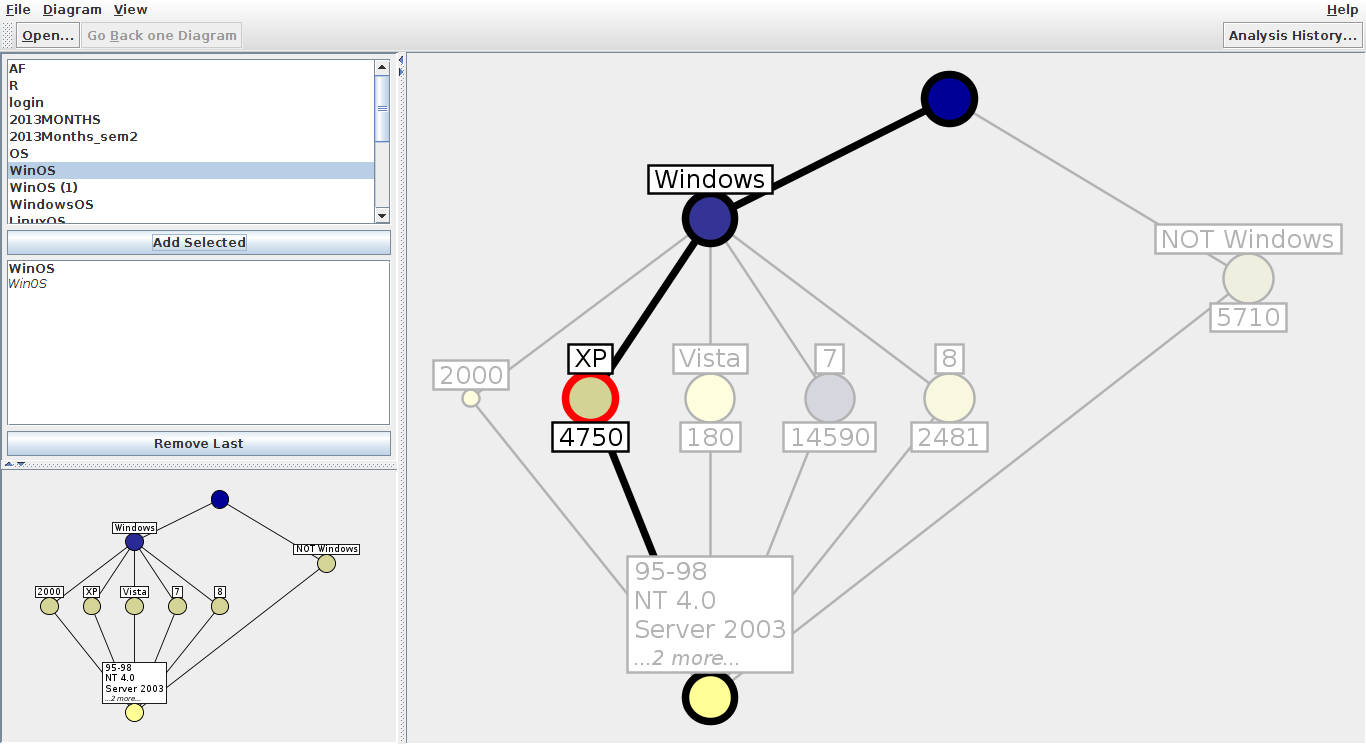
\includegraphics[width=\textwidth, natwidth=1366, natheight=744]{toscanaj-1.png} \\ 
          \caption{ToscanaJ, afișând o latice simplă generată din date de acces ale unui site web}
          \label{screenshot:toscana-1}
        \end{figure}
        \begin{figure}[h]
          \centering
          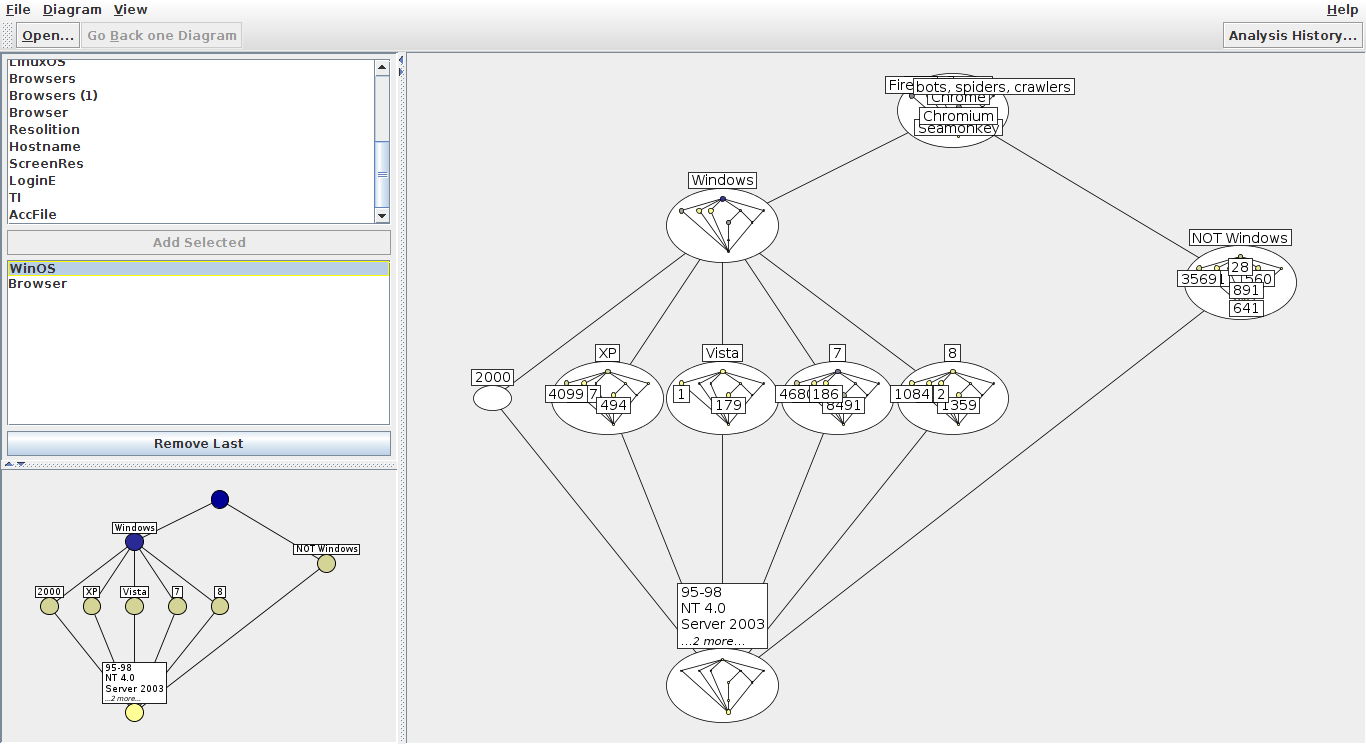
\includegraphics[width=\textwidth, natwidth=1366, natheight=744]{toscanaj-2.png}
          \caption{ToscanaJ, afișând aceeași latice ca în \ref{screenshot:toscana-1}, de data aceasta imbricată cu altă diagramă}
          \label{screenshot:toscana-2}
        \end{figure}

        Interfața ToscanaJ este punctul de pornire pentru Romagna. Vom încerca să păstrăm anumite elemente comune, pentru a ajuta utilizatorii obișnuiți, dar vom face, bine-nțeles schimbări și adaptări, mai ales luând în considerare diferențele convențiilor dintre interfețele aplicațiilor web, și cele desktop.

        ToscanaJ este, asemenea Romagna, doar un navigator de concepte. Modelarea conceptelor din date este realizată cu ajutorul altor programe din suita din care face parte și ToscanaJ.

        \begin{description}
            \item[Elba] este un editor pentru schemele conceptuale, legat de baze de date.
            \item[Siena] este un editor pentru scheme conceptuale, foarte asemănător cu \textbf{Elba}, diferența fiind că Siena nu are nevoie de o legătură cu o bază de date, putând descrie concepte simple direct în program.
        \end{description}

  \subsection{GaloisExplorer}
    GaloisExplorer \cite{GaloisExplorer:homepage} este un program mai recent, cu ultima actualizare în 2009.

    Are o intefață realizată în QT, ceea ce îi permite să funcționeze pe mai multe platforme. O abordare interesantă, dar în cele din urmă doar cu valoare estetică, este prezentarea laticelor în 3d (\ref{screenshot:galoisexplorer}).
   
    Din păcate, folosește anumite librării 3d (coin3d\cite{Coin:homepage}) care nu sunt imediat disponibile și care necesită compilare manuală.

    Pentru mulți utilizatori care nu au cunoștințe avansate de calculatore, aceste impedimente sunt motiv suficient pentru a abandona această instalare.
    \begin{figure}[h]
      \centering
      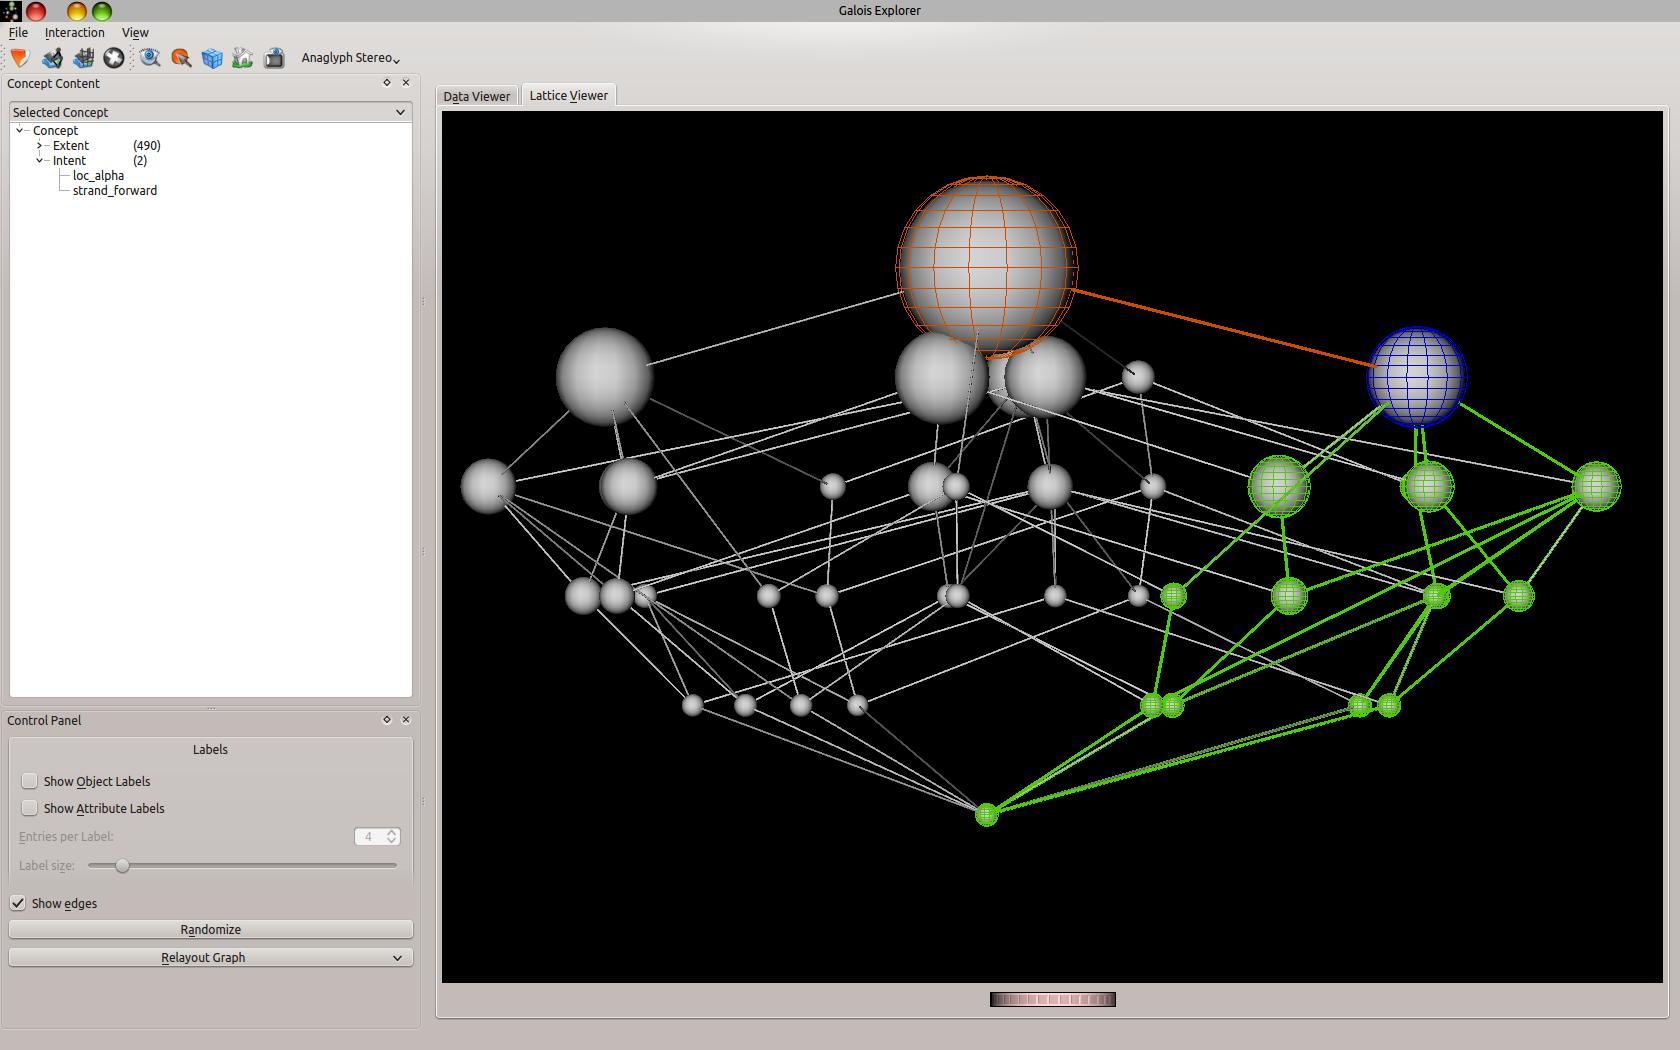
\includegraphics[width=\textwidth]{GaloisExplorer_latticeView}
      \caption{GaloisExplorer, afișând o diagramă în 3d. Sursa: site-ul proiectului \cite{GaloisExplorer:sourceforge}}
      \label{screenshot:galoisexplorer}
    \end{figure}

  \section{Software conex}
  %TODO: define Duquenne-Guiges
  %TODO: schimbă traducerile trimise de prof

    În această secțiune vom prezenta câteva alte programe remarcabile în domeniul FCA, sau care au avut un impact indirect asupra dezvoltării Romagna:
    \begin{description}
      \item[FCAStone] dezvoltat de Uta Priss, e un program care urmărește obținerea inter-operabilității între diferite programe pentru FCA (numele vine de la Piatra \textit{[n.t. Stone = Piatră]} Rosetta) și convertește contexte în latice de concepte, și latice de concepte în formate grafice.
      \item[Conexp] dezvoltat de Serhiy A. Yevtushenko, este o unealtă scrisă în Java, folosită în principal în scopuri educaționale (dar nu numai), are numeroase funcționalități de modelare a contextelor, dintre care amintim:
        \begin{itemize}
            \item calculează numărul de concepte formale dintr-un context dat
            \item calculează laticea de concepte
            \item permite explorarea atributelor
            \item calculează mulțimea de implicații Duquenne-Guiges
            \item calculează regulile de asociații
        \end{itemize}
      \item[\LaTeX for FCA] \cite{LatexForFCA:homepage} Plugin pentru \LaTeX, scris de Bernhard Ganter, oferă câteva ``environment''-uri noi, folosite și în această lucrare, care permite aranjarea ușoară în pagina a contextelor și a laticilor derivate din acestea.
    \end{description}

\chapter{Romagna}

  Romagna este o aplicație dezvoltată începând cu anul 2014, pornită la Universitatea Babeș-Bolyai ca o alternativă folosindu-se de tehnologiile web pentru un navigator de concepte modern.


  \section{Raționament}
  \label{sec:rationament}

    \subsection{Ușurință de utilizare}

    \subsection{Avantajele distribuirii aplicațiilor web}

    \subsection{Folosirea web-ului, păstrarea confidențialității datelor}
  \section{Structură}
  \section{Tehnologii}
    \subsection{CoffeeScript}
    \subsection{Ember.js}
    \subsection{d3.js}
      \subsubsection{svg}
    \subsection{sql.js}
      \subsubsection{emscripten}
        Emscripten e super mișto pentru că te lasă să compilezi programe scrise în C/++ în JavaScript... TO BE CONTINUED

  \section{Dezvoltare}

    \subsection{Proces}

    \subsection{Probleme întâmpinate}
      \subsubsection{MySQL versus sql.js} % (fold)
      \label{ssub:MySQL versus sql.js}

      % subsubsection MySQL versus sql.js (end)
      \subsubsection{SVG IS FUCKED}

    \subsection{Viitor}
  \chapter{Concluzii}

\bibliographystyle{alpha}
\bibliography{romagna}
\appendix
\end{document}
